
Each of the once-through transition scenarios are compared on multiple 
criteria: the number of advanced reactors deployed, \hl{the energy profile?}, 
the mass of enriched 
uranium required, the amount of \gls{SWU} capacity required to enrich uranium,
and the mass of waste produced. A subset of these results are presented
in \cite{bachmann_enrichment_2021}, except the \glspl{LWR} were assumed to 
operate for 60 years if not closed before December 2020. The results of Scenario 
1 are presented first, followed by the results of the no growth scenarios 
(Scenarios 2-7), then the results of the 1\% growth scenarios (Scenarios 8-13). 

\section{Scenario 1}
Scenario 1 models only the \glspl{LWR} deploying the United States with no 
perscribed energy demand. Figure \ref{fig:reactor1} shows the number of 
reactors deployed in Scenario 1 as a function of time. A maximum of 109 
\glspl{LWR} are deployed at one time in this scenario, and 92 \glspl{LWR}
are deployed when the transition begins in 2025. All of the \glspl{LWR} are
decommissioned by October of 2055. 

\begin{figure}
    \centering
    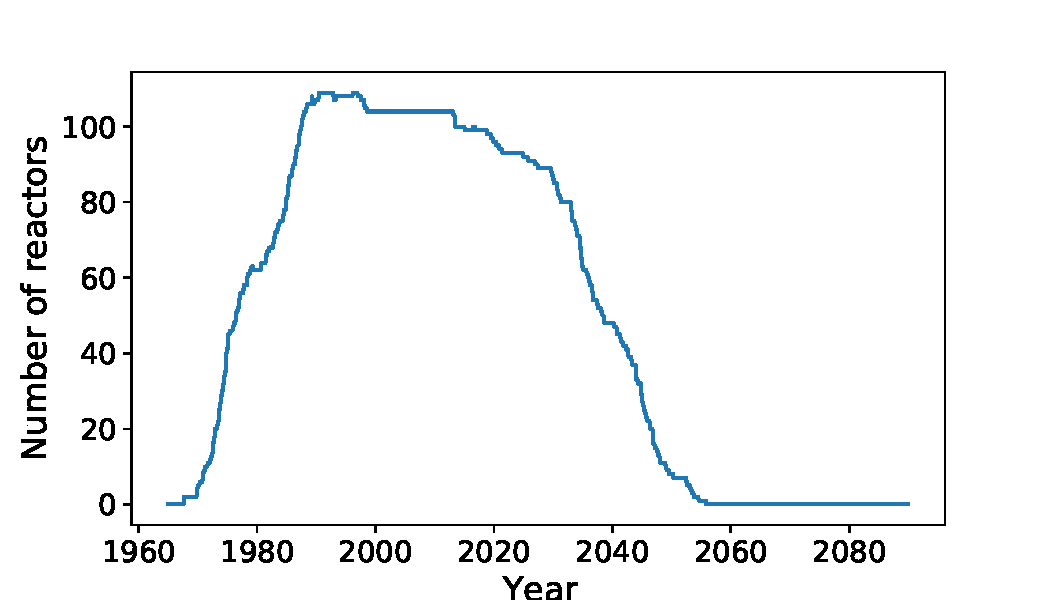
\includegraphics[scale=0.8]{s1_reactors.pdf}
    \caption{Number of LWRs deployed at each time step in Scenario 1.}
    \label{fig:reactor1}
\end{figure}

The mass of enriched uranium sent to the \glspl{LWR} in this scenario (Figure 
\ref{fig:fuel1}) follows the general pattern of the reactor deployment, but with 
more variation between individual time steps. The increased variation between 
time steps is becuase of the staggering of outages for the reactors, or when 
they receive fuel. There are also times with large increases in the mass of fuel 
sent to the reactore, such as in 2016, because these times include the deployment 
of a new reactor with a full core of fuel instead of the amount that is 
sent for refueling. 

The maximum amount of enriched uranium sent to the \glspl{LWR} at any one 
time in this scenario is 513.72 MTU. The average mass of enriched uranium sent to 
the reactors for the entire scenario is 95.65 MTU/month. The average mass of 
uranium sent to \glspl{LWR} between 2025-2055, from the start of the transition 
to when they are all decommissioned is 81.11 MTU/month. 

\begin{figure}
    \centering
    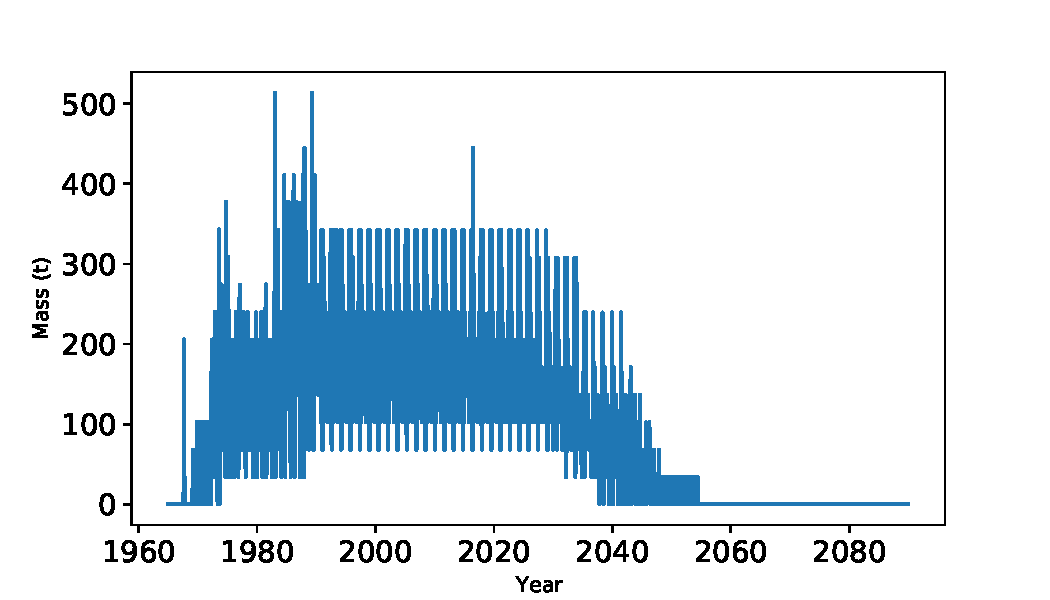
\includegraphics[scale=0.8]{s1_fuelsupply.pdf}
    \caption{Mass of uranium supplied to the LWRs in Scenario 1 at each time step.}
    \label{fig:fuel1}
\end{figure}

The mass of natural uranium required to produce the fuel sent to the reactors at 
is about an order of magnitude larger than the mass of the enriched uranium 
(Figure \ref{fig:feed1}). 

\begin{figure}
    \centering
    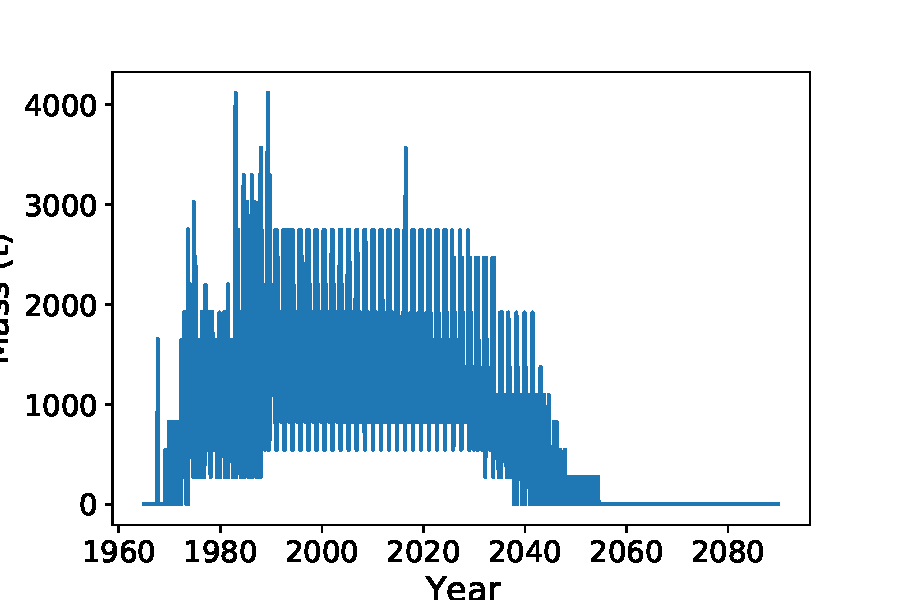
\includegraphics[scale=0.8]{s1_feed.pdf}
    \caption{Mass of natural uranium required to supply the fuel sent to LWRs at each time step in Scenario 1.}
    \label{fig:feed1}
\end{figure}

A maximum of 3.7$\times 10^6$ kg-SWU is required to 
enrich the uranium sent to the reactors at one time step. An averge of 
0.69$\times 10^6$ kg-SWU/month is needed to enrich all of the uranium sent to 
the \glspl{LWR}, and an averge of 0.59$\times 10^6$ kg-SWU/month is needed to 
enriched the uranium sent to \glspl{LWR} between 2025 and 2055.


\begin{figure}
    \centering
    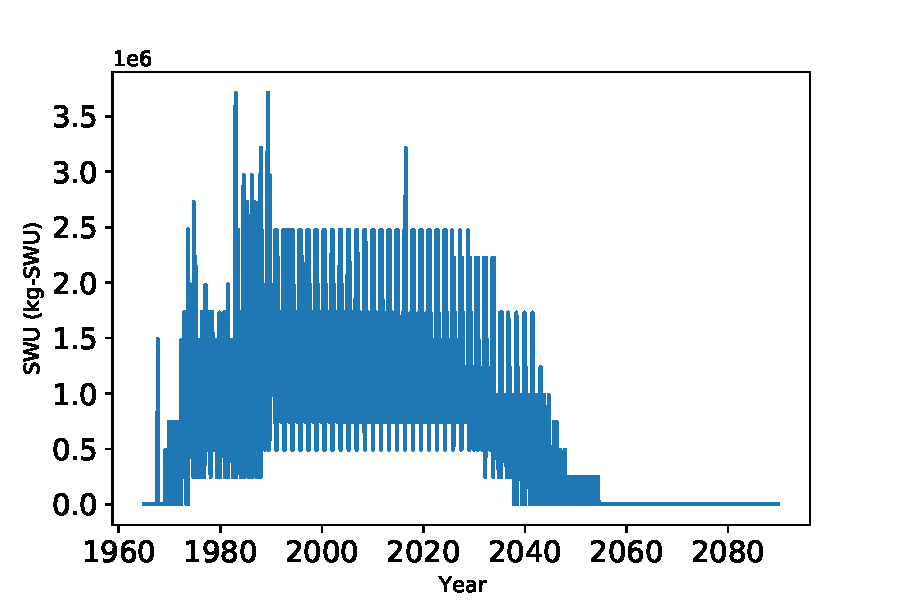
\includegraphics[scale=0.8]{s1_swu.pdf}
    \caption{SWU capacity required to enrich the uranium sent to LWRs at each time step in Scenario 1.}
    \label{fig:swu1}
\end{figure}

Finally, the waste discharged from the reactors as a function of time is shown 
in Figure \ref{fig:waste1}. An maximum of 410.29 MT of spent fuel is discharged 
from the \glspl{LWR} at one time step. An average of 95.65 MT/month of spent fuel is 
discharged from the reactors across the entire simulation, and an average of 
106.63 MT/month of spent fuel is discharged from reactors between 2025-2055. 

\begin{figure}
    \centering
    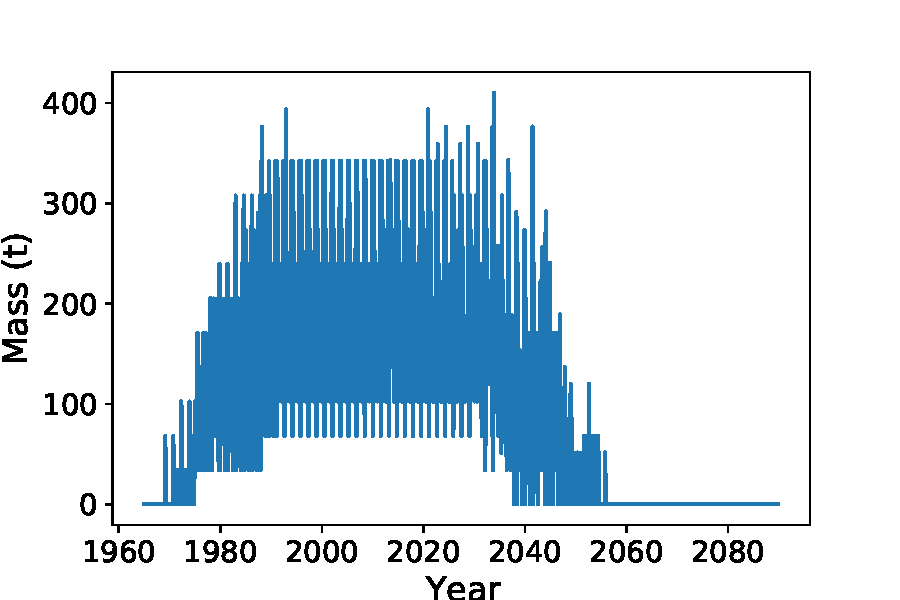
\includegraphics[scale=0.8]{s1_waste.pdf}
    \caption{Mass of spent fuel dishcarged from the reactors in Scenario 1 as a function of time.}
    \label{fig:waste1}
\end{figure}

\section{Reactor deployment}
Each of the scenarios are compared on the number of advanced reactors that must 
be built to meet the prescribed energy demand. 
\subsection{No growth scenarios}

\begin{figure}
    \centering
    \includegraphics[scale=0.8]{nogrowth_reactors.pdf}
    \caption{Total number of advanced reactors as a function of time in Scenarios 2-7.}
    \label{fig:nogrowth_reactors}
\end{figure}

\begin{table}
    \centering 
    \caption{Maximum number of each type of advanced reactor and maximum total 
    number of reactors deployed in Scenarios 2-7}
    \label{tab:reactors_nogrowth}
    \begin{tabular}{c c c c c}
        \hline
        Scenario & \glspl{MMR} & Xe-100s & VOYGRs & Total\\\hline
        2 & 9182 & - & - & 9182\\
        3 & - & 1225 & - & 1225\\
        4 & 752 & 1124 & - & 1876\\
        5 & 127 & - & 1811 & 1938\\
        6 & - & 1099 & 191 & 1288\\
        7 & 782 & 1122 & 0 & 1902\\
        \hline
    \end{tabular}
\end{table}

\begin{table}
    \centering 
    \caption{Maximum number of each type of advanced reactor and maximum total 
    number of reactors added to the simulation at a single time step in Scenarios 2-7.}
    \label{tab:reactors_added_nogrowth}
    \begin{tabular}{c c c c c}
        \hline
        Scenario & \glspl{MMR} & Xe-100s & VOYGRs & Total\\\hline
        2 & 378 & - & - & 378\\
        3 & - & 50 & - & 50\\
        4 & 31 & 50 & - & 56\\
        5 & 4 & - & 75 & 78\\
        6 & - & 49 & 8 & 51\\
        7 & 30 & 50 & 0 & 56\\
        \hline
    \end{tabular}
\end{table}

\subsection{1\% growth scenarios}

\begin{table}
    \centering 
    \caption{Maximum number of each type of advanced reactor and maximum total 
    number of reactors deployed in Scenarios 8-13}
    \label{tab:reactors_1growth}
    \begin{tabular}{c c c c c}
        \hline
        Scenario & \glspl{MMR} & Xe-100s & VOYGRs & Total\\\hline
        8 & \\
        9 & \\
        10 & \\
        11 & \\
        12 & \\
        13 & \\
        \hline
    \end{tabular}
\end{table}

\section{Uranium resources}

\subsection{No growth scenarios}

\subsection{1\% growth scenarios}

\section{SWU capacity}
\subsection{No growth scenarios}

\subsection{1\% growth scenarios}

\section{Waste}
\subsection{No growth scenarios}

\subsection{1\% growth scenarios}